
\section{Geometric Details}
\label{sec:app_geometry}

This appendix spells out the geometric quantities that the main text defers, so that Section~\ref{sec:method} stays readable while the construction in Eqs.~\ref{eq:lift}--\ref{eq:lat-update} remains fully reproducible.

\boldstart{Conventions.}
Extrinsics $\mathbf{E}_t \in \mathrm{SE}(3)$ map world points into camera $t$, and we denote the camera-to-world inverse by $\mathbf{E}_t^{-1}$.
Intrinsics follow the standard pinhole form with focal lengths $(f_x, f_y)$ and principal point $(c_x, c_y)$.
The VAE has spatial stride $s$ dividing the pixel resolution $H \times W$ into the latent resolution $h \times w = (H/s) \times (W/s)$, with $s = 16$ throughout (Appendix~\ref{sec:app_implementation}).
Latent cells are indexed by $(u, v) \in \{0, \dots, w-1\} \times \{0, \dots, h-1\}$ with pixel-centre homogeneous coordinates $[u + \tfrac{1}{2}, v + \tfrac{1}{2}, 1]^\top$.

\boldstart{Latent-resolution intrinsics.}
The latent-resolution intrinsic matrix used in Eqs.~\ref{eq:lift} and~\ref{eq:read} is obtained from the pixel-resolution intrinsics $K$ by scaling both axes by the corresponding stride ratio,
\begin{equation}
K^{\ell} = \mathrm{diag}(w/W,\, h/H,\, 1)\, K.
\end{equation}
Both focal lengths and the principal point are rescaled by the same per-axis ratio, so that perspective projection remains consistent after the depth map is downsampled to latent resolution.
In the main text we slightly abuse notation by writing $K$ for $K^{\ell}$ wherever the context is unambiguous.

\boldstart{Pinhole back-projection.}
The operator $\pi^{-1}$ used in Eq.~\ref{eq:lift} maps a latent cell $(u, v)$ with depth $d = D(u, v)$ into a world point through ray-casting in camera coordinates followed by the camera-to-world transform,
\begin{equation}
\pi^{-1}(u, v, d;\, K^{\ell}, \mathbf{E}) = \mathbf{E}^{-1}\!\begin{bmatrix} d\,(K^{\ell})^{-1} [u + \tfrac{1}{2},\, v + \tfrac{1}{2},\, 1]^\top \\ 1 \end{bmatrix}\Biggl.\Biggr|_{1:3},
\end{equation}
where the trailing subscript denotes selection of the first three coordinates.

\boldstart{Projection onto the latent grid.}
For a memory point $\mathbf{p}_i$, its camera-space position at target view $t$ is the first three coordinates of $\mathbf{E}_t [\mathbf{p}_i^\top, 1]^\top$, which we denote $\mathbf{q}_i \in \mathbb{R}^3$.
Its position on the latent grid is then
\begin{equation}
\pi^{\ell}(\mathbf{q}_i) = \bigl(\lfloor x \rfloor, \lfloor y \rfloor\bigr), \qquad [x, y, 1]^\top = K^{\ell}\, \mathbf{q}_i / [\mathbf{q}_i]_z.
\end{equation}
The candidate set used in the readout of Eq.~\ref{eq:read} is then
\begin{equation}
\Omega_t(u, v) = \bigl\{ i : \pi^{\ell}(\mathbf{q}_i) = (u, v),\; [\mathbf{q}_i]_z > 0 \bigr\},
\end{equation}
and the admissible cell set $\Lambda_t$ in Eq.~\ref{eq:lat-update} is defined on the same grid, restricted to cells with finite positive depth that lie outside the dynamic-object and sky masks.


\section{Additional Experimental Analysis}
\label{sec:app_experiment}

\begin{figure*}
    \centering
    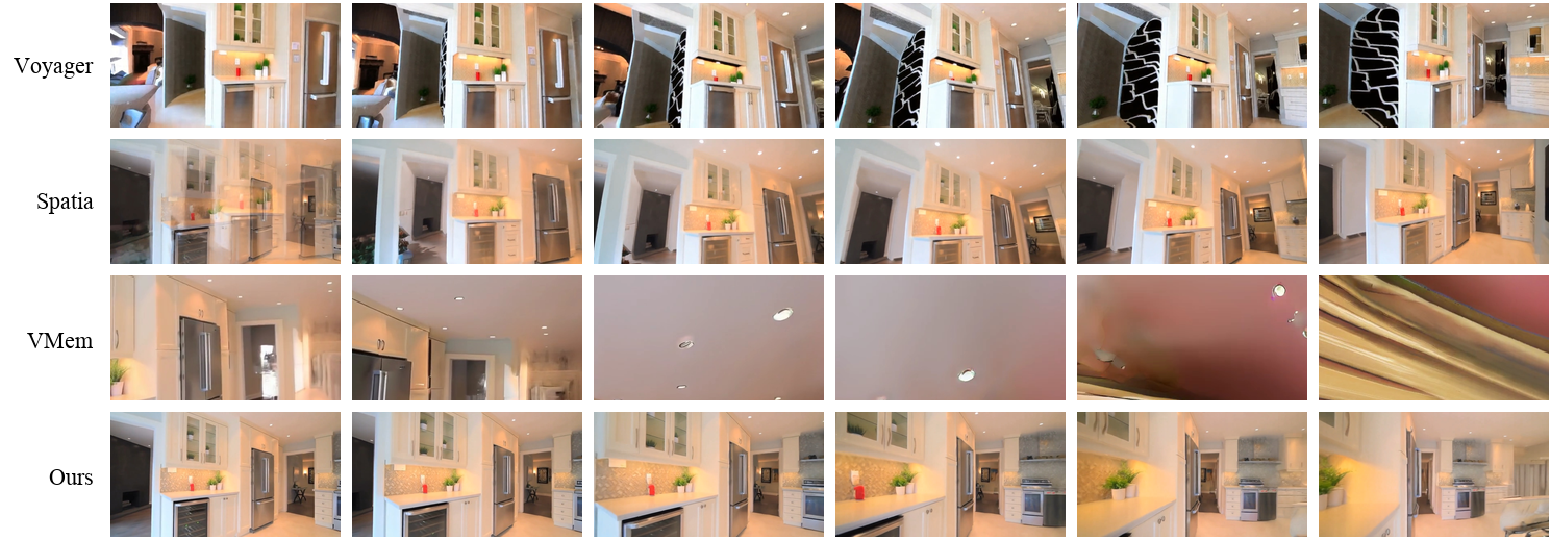
\includegraphics[width=1.0\textwidth]{figures/re10k2.pdf}
    \caption{\textbf{Additional video comparison on a challenging indoor trajectory.}
    \method{} maintains coherent layout  over the full trajectory, whereas baselines suffer from view-dependent deformation, blur, and inconsistent scene reconstruction.
    }

    \label{fig:re10k_video_2}
\end{figure*}

This appendix complements Section~\ref{sec:exp} with analyses that clarify \emph{why} latent spatial memory is efficient, \emph{how} it behaves as the rollout horizon grows, and \emph{what} the stored tokens carry compared with an RGB cache.

\boldstart{Asymptotic cost of cache reads.}
Let $N$ denote the cache size at a given step.
Reading an RGB cache costs $\Theta(N \log N + HW) + \Theta(\Phi_\mathcal{E}(H, W))$ per conditioning step, where $\Phi_\mathcal{E}$ is the FLOP count of one VAE encoder pass.
Reading a latent cache costs $\Theta(N \log N + hw)$: the rasterisation term shrinks by the squared VAE stride, and the per-step encoder term disappears entirely because the readout is already in the backbone's input space.
The peak memory of the cache itself follows the ratio $s^2 \cdot (3 / C)$ between the RGB and latent representations, which together with the per-step pixel-resolution buffer accounts for the order-of-magnitude gap reported in Figure~\ref{fig:efficiency_scaling}.
The gap widens with the rollout horizon: the $N \log N$ sort begins to dominate the latent cache much later than the pixel cache, and the RGB baseline exhausts GPU memory on trajectories that \method{} completes comfortably.

\boldstart{Per-step timing breakdown.}
We decompose the per-step cost of the RGB pipeline into rasterisation, VAE encoder forward, and depth estimation plus back-projection.
On a $257$-frame rollout, rasterisation and the encoder together account for more than $98\%$ of the per-step RGB cost, and both are absent from the conditioning loop of \method{}, since a single latent-resolution projection replaces them.
The decoder, which the RGB pipeline calls at every conditioning step to produce the image on which the cache is rasterised, is invoked in \method{} only once per chunk to materialise output frames and to feed the depth and segmentation modules; it never appears on the per-step critical path.

\boldstart{Depth down-sampling for cache construction.}
Eq.~\ref{eq:lift} requires the dense depth map and the latent grid to share a resolution, so depth must be down-sampled before lifting.
Because depth is piecewise smooth with discontinuities at silhouettes, this choice is not neutral: bilinear interpolation smears foreground over background at edges and can spawn phantom points; nearest-neighbour preserves edges but aliases fine structure; area pooling over-smooths occluding contours; median pooling preserves edges but is biased on slanted surfaces.
We evaluate all four with every other component fixed.
Table~\ref{tab:depth_down} reports the fraction of empty latent cells in the projected cache (``hole rate'').
Among the four down-sampling choices, bilinear interpolation gives the lowest hole rate at $42.53\%$.
We therefore adopt bilinear as the default, since it provides the best projected-cache coverage among the tested variants.

\begin{table}[t]
    \centering
    \caption{\textbf{Depth down-sampling for cache construction.} Evaluated on a held-out RealEstate10K split with every other component of \method{} kept fixed.}
    \label{tab:depth_down}
    \begin{tabular}{lc}
    \toprule
    Down-sampling $D \to D^{\ell}$ & Hole Rate $\downarrow$ \\
    \midrule
    Bilinear (default) & 42.53 \\
    Nearest-neighbour  & 47.78 \\
    Area pooling       & 53.72 \\
    Median pooling     & 52.22 \\
    \bottomrule
    \end{tabular}
\end{table}

\boldstart{What the cache stores.}
The latent tokens are expected to carry semantic and textural structure that three color channels cannot express.
We visualize this by projecting each per-point feature vector onto its top three principal components and coloring the memory by the resulting RGB.
Coherent semantic clusters such as walls, floors, windows, and furniture emerge that are not recoverable from an RGB point cloud built on the same frames.
This is the qualitative mechanism behind Table~\ref{tab:ablation}, where swapping the latent cache for an RGB cache with the backbone and training recipe held fixed weakens both 3D and photometric consistency.


\section{Implementation Details}
\label{sec:app_implementation}

\boldstart{Backbone and latents.}
The backbone is Wan2.2-TI2V-5B~\cite{wan2025wan}, whose VAE has spatial stride $s = 16$, temporal stride $4$, and channel count $C = 48$.
Each generation chunk covers a $9 \times 44 \times 80$ latent tensor corresponding to $33$ RGB frames at $704 \times 1280$.
The transformer has hidden dimension $3072$, feed-forward dimension $14336$, $24$ attention heads, $30$ blocks, text context $512$ tokens, and uses RMS Q/K normalisation together with cross-attention normalisation.
The VAE is frozen throughout.

\boldstart{Conditioning branch.}
The latent readout $\hat{\mathbf{z}}_t$ is injected through a ControlNet-style side branch whose layout mirrors the VACE~\cite{jiang2025vace} blocks of Wan2.2 and shares its patch embedding with the main network.
The branch is attached at layers $\{0, 4, 8, 12, 16, 20, 24, 28\}$ with a $48$-channel input matching the VAE latent, so no bridging encoder is required.
Segment-aware rotary positional encoding~\cite{su2024roformer} tags each frame as noisy target, clean preceding, or clean reference inside a single forward pass; at inference, the denoised latents of the previous chunk become the preceding frames of the next.

\boldstart{Training.}
Training has two flow-matching~\cite{lipman2022flow} stages on the target frames.
Stage one updates only the side branch at learning rate $10^{-5}$ with the backbone and VAE frozen.
Stage two unlocks rank-$64$ LoRA adapters~\cite{hu2021lora} on the $\{\texttt{q}, \texttt{k}, \texttt{v}, \texttt{o}\}$ projections of every self-attention layer ($\alpha = 64$, dropout $0.05$) and jointly optimises them with the side branch at learning rate $10^{-4}$.
Optimisation uses AdamW ($\beta = (0.0, 0.999)$, weight decay $10^{-3}$), a cosine schedule, bfloat16 mixed precision under FSDP sharding, gradient checkpointing, and text-dropout probability $0.2$.
At inference we use the UniPC flow scheduler with $40$ steps and classifier-free guidance disabled; efficiency is reported on a single NVIDIA H100.

\boldstart{Data.}
Training clips are drawn from RealEstate10K.
Each clip is processed by a feed-forward reconstructor~\cite{lin2025depth} for metric depth, intrinsics, and per-frame extrinsics, and by a Qwen3-VL-2B~\cite{yang2025qwen3} entity extractor followed by SAM3~\cite{carion2025sam3segmentconcepts} for foreground-dynamic and sky masks.
Cells inside the mask are excluded from $\Lambda_t$ in Eq.~\ref{eq:lat-update} so that only geometry compatible with the rigid-scene assumption enters the persistent memory.
Frames, latents, depth, and camera parameters are stored in an LMDB-backed dataset, so no re-encoding occurs during training.
Rollouts are produced in chunks of nine latent frames with one-frame overlap to preserve temporal continuity, and the cache is grown once per chunk by re-encoding the decoded frames and lifting them via Eq.~\ref{eq:lift}.
Algorithm~\ref{alg:latmem} summarises one complete rollout.

\begin{algorithm}[t]
\caption{One rollout of \method{}.}
\label{alg:latmem}
\begin{algorithmic}[1]
\Require initial frame $I_0$; camera trajectory $\{(\mathbf{E}_t, K_t)\}_{t=0}^{T}$ with $\mathbf{E}_0$ fixed to the world frame
\State $\mathbf{z}_0 \leftarrow \mathcal{E}(I_0)$
\State $D_0 \leftarrow \textsc{DepthAnything3}(I_0)$
\State $M_0 \leftarrow \textsc{SAM3}(\textsc{Qwen3-VL}(I_0)) \cup \textsc{sky}(I_0)$
\State $\mathcal{M} \leftarrow \{(\mathbf{p}_{uv}, \mathbf{f}_{uv}) : (u, v) \in \Lambda_0\}$ via Eq.~\ref{eq:lift} on $(\mathbf{z}_0, D_0, K_0, \mathbf{E}_0)$
\State $\tau \leftarrow 0$; $\mathcal{O} \leftarrow \{I_0\}$ \Comment{collected output frames}
\While{$\tau < T$}
    \State sample latent chunk $W = \{\tau + 1, \dots, \tau + |W|\}$
    \For{$t \in W$} \Comment{read at latent resolution}
        \State $\hat{\mathbf{z}}_t, \mathbf{m}_t \leftarrow$ readout of $\mathcal{M}$ at $(\mathbf{E}_t, K_t)$ via Eq.~\ref{eq:read}
    \EndFor
    \State $\{\mathbf{z}_t\}_{t \in W} \leftarrow$ backbone$\bigl(\{\hat{\mathbf{z}}_t, \mathbf{m}_t\}_{t \in W}, \text{preceding}, \text{reference}\bigr)$
    \For{$t \in W$} \Comment{decode-and-re-encode update, once per chunk}
        \State $I_t \leftarrow \mathcal{D}(\mathbf{z}_t)$; append $I_t$ to $\mathcal{O}$
        \State $D_t \leftarrow \textsc{DepthAnything3}(I_t)$
        \State $M_t \leftarrow \textsc{SAM3}(\textsc{Qwen3-VL}(I_t)) \cup \textsc{sky}(I_t)$
        \State $\tilde{\mathbf{z}}_t \leftarrow \mathcal{E}(I_t)$
        \State $\mathcal{M} \leftarrow \mathcal{M} \cup \{(\mathbf{p}_{uv}, \mathbf{f}_{uv}) : (u, v) \in \Lambda_t\}$ via Eq.~\ref{eq:lift} on $(\tilde{\mathbf{z}}_t, D_t, K_t, \mathbf{E}_t)$
    \EndFor
    \State $\tau \leftarrow \tau + |W|$
\EndWhile
\State \Return $\mathcal{O}$
\end{algorithmic}
\end{algorithm}






